\subsection{Variable coefficients}

In this part, we will change the equation a little and add variable coefficients so that the equation becomes : 
$$q_t = a(y)q_{xx}+b(x)q_{yy}+S$$
\subsubsection{Finite volume method}

Using the same principles as in section 3, we get the following :
$$\frac{1}{\Delta x \Delta y} \iint_{(i,j)} q_tdxdy = \frac{1}{\Delta x \Delta y} \iint_{(i,j)} \nabla \cdot \left(\begin{array}{c}
a(y)q_x \\ 
b(x)q_y
\end{array}\right) dxdy + \frac{1}{\Delta x \Delta y}\iint_{(i,j)}Sdxdy $$ 
$$\frac{dQ_{ij}}{dt} = \frac{1}{\Delta x \Delta y}(\int_E a(y)q_xdy + \int_N b(x)q_ydx - \int_Wa(y)q_xdy - \int_S b(x)q_ydx) + S_{ij}$$

Using finite differences to evaluate $q_x$ and $q_y$, we get : 
$$\frac{dQ_{ij}}{dt} = E\frac{aQ_{i+1,j}+bQ_{i,j}+cQ_{i-1,j}}{\Delta x^2}+F\frac{dQ_{i,j+1}+eQ_{i,j}+fQ_{i,j-1}}{\Delta y^2}+S_{ij}$$

Where $a,b,c,d,e,f$ are the same coefficients as those defined in section 3.1. $E$ and $F$ take into account the variable coefficient and are defined by : 
$$E = \frac{1}{\Delta y}\int_E a(y)dy= \frac{1}{\Delta y}\int_W a(y)dy$$
$$F = \frac{1}{\Delta x}\int_N b(x)dx= \frac{1}{\Delta x}\int_S b(x)dx$$

So, if we use the same notations as in section 3.1, the only thing we have to do is premultiply $B$ and $C$ with the corresponding matrix and after that, the implementation is unchanged. We can note that if $a(y)=b(x)=1$ then $E$ and $F$ are identity matrices and we have the same rule as previously.

In this problem, we have always used the smooth source term. We also have used the trapezoidal rule to evaluate the integral. Let us define $A1$ the $n \times n$ matrix as :
$$A1 = diag(0.5(a(0)+a(\Delta y)),0.5(a(\Delta y)+a(2\Delta y)),...,0.5(a((n-1)\Delta y)+a(1)))$$

Which is a diagonal matrix containing the different evaluations of the integral of $a$. With this matrix, we can build $B1$ as :
$$B1 = (A1\otimes I(m))*B$$

Identically, we can define $A2$ as :
$$A2 = diag(0.5(b(0)+b(\Delta x)),0.5(b(\Delta x)+b(2\Delta x)),...,0.5(b((m-1)\Delta x)+b(1)))$$

And then : 
$$C1 = (I(n)\otimes A2)*C$$
And finally : 
$$M = B1 + C1$$

Once we have build $M$, the methodology is exactly the same as before. We get the following ODE's system :
$$\frac{dQvect}{dt} = MQvect + S$$

And we can use the same technique as in section 3.

The implementation of the method is done in $variableCoeff.m$.

\subsubsection{Plots, convergence and conservation}
The matlab code called $varCoeffConv.m$ plots the solution and returns the order of convergence for space and time.

For our implementation, we have used the following function $a$ and $b$ : 
$$a(y) = y$$
$$b(x) = x$$

\begin{figure}[!htb]
\centering
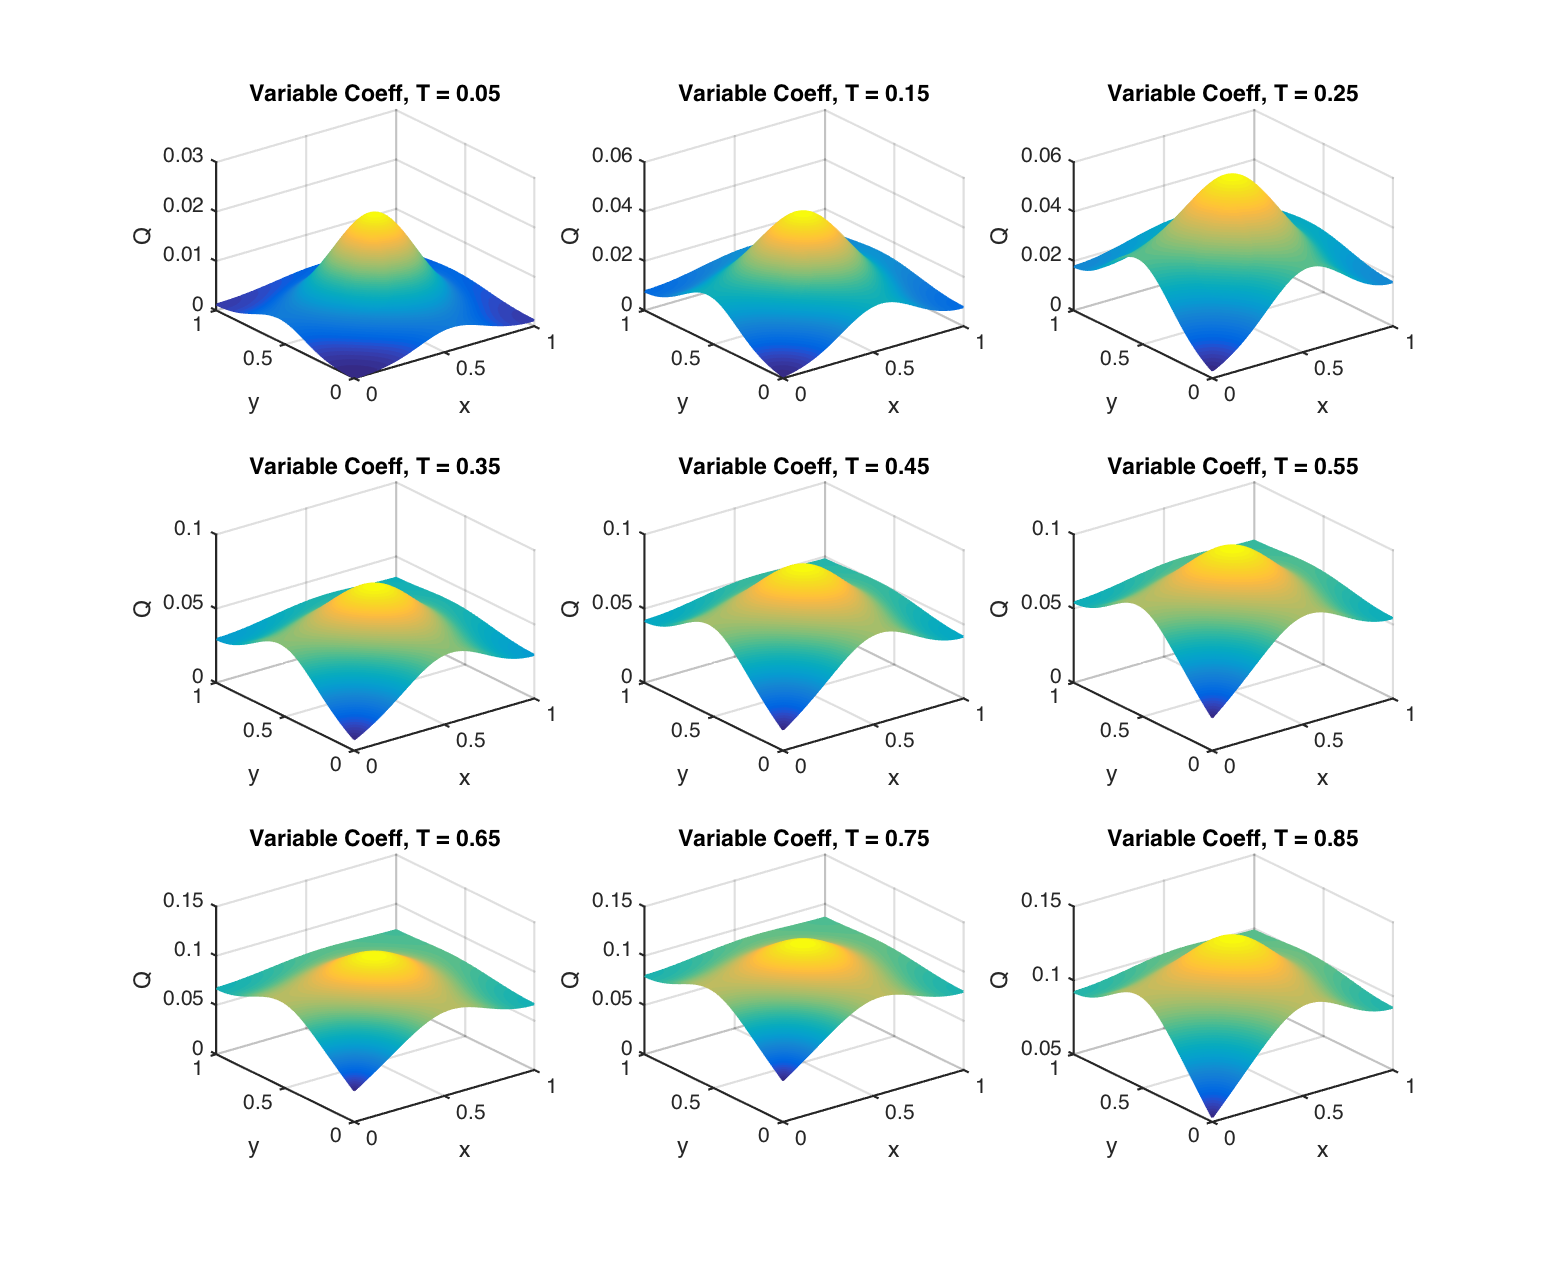
\includegraphics[scale=.6]{varCoeff.eps}
\caption{Results with Variable Coefficients}
\label{fig:digraph}
\end{figure}
Figure (5) shows the solution for different times. We can see that at first the source term is dominant. After that, it is the conduction. The functions $a$ and $b$ can be seen as the conduction coefficients. The higher they are, the quicker the heat will travel in that direction. It is easily seen in the plots. Heat "has trouble" reaching $(0,0)$ because there $a$ and $b$ are small. On the other end, where $a$ and $b$ are close to one, the conduction is really quick.

Let us now look at the convergence. The code used, $varCoeffConv.m$, is available at the end of the report.

First, the spatial convergence. Let us define :
$$R = log_2(\frac{Q_h-Q_{h/2}}{Q_{h/2}-Q_{h/4}})$$

Where $Q_h$ is our solution evaluated at $(1,1)$ (the last cell) at $t=1$ for a grid such that $h=\Delta x= \Delta y$.

Our code gives the following values : 
\begin{center}
\begin{tabular}{|c|c|c|c|}
\hline 
h & $\frac{1}{40}$ & $\frac{1}{80}$ & $\frac{1}{160}$ \\ 
\hline 
R & 1.9953 & 1.9991 & 1.9999 \\ 
\hline 
\end{tabular} 
\end{center}

We can see that the value seems to converge to 2. Hence, we can conclude that the order of spatial convergence is 2.

Let us now look at the time convergence. Let us define :
$$H = log_2(\frac{Q_{\Delta t}-Q_{\Delta t/2}}{Q_{\Delta t/2}-Q_{\Delta t/4}})$$

Where $Q_{\Delta t}$ is our solution evaluated at $(1,1)$ and $t=0.4$ and $m=n=200$ with the time step $\Delta t$. This yields the results : 
\begin{center}
\begin{tabular}{|c|c|c|c|}
\hline 
$\Delta t$ & 0.08 & 0.04 & 0.02 \\ 
\hline 
H & 1.0680 & 0.9884 & 0.9801 \\ 
\hline 
\end{tabular} 
\end{center}

So we can conclude that the order of convergence is 1. This is to be expected since implicit Euler is used.\\

Let us finally look at the conservation. Our code returns the absolute value of the difference between the total heat given to the system by the heat source and the heat contained in the system at final time. Because the walls are insulated, those two values should be equal.

Running our code with $m=n=400$, $\Delta t = 0.01$ and the final time being 0.5, we get that the difference $\Delta heat$ is :
$$\Delta heat = 5.6150 * 10^{-14}$$

Which is very close to zero and should be considered as such. We have thus verified that our scheme is numerically conservative.

\subsection{Boundary conditions}
We are now going to try and change the boundary conditions to see what happens. We have a Neuman condition on the left and right boundaries (just as before except it is no longer homogeneous). And we now have a Dirichlet condition on the upper and lower boundaries. Because in the previous grid, we had no point exactly on the boundary, we are going to shift the grid of $\frac{\Delta y}{2}$ in the y-direction. That way, we will have center of cells at $y=0$ and $y=1$. If we still keep $n\Delta y =1$, that means that we will now have $m(n-1)$ unknowns since the value on the upper and lower boundaries are known.

\subsubsection{Finite volume method}
We use the same methodology as before. We rewrite $Q$ as $Qvect$ and we will show that we will get a system of ODE's of the following type : 
$$\frac{dQvect}{dt} = A_xQvect+A_yQvect+b_x+b_y+S$$

We already know the definition of $S$, it is unchanged. $A_x$ and $b_x$ represents the derivative in the x-direction ($b_x$ is not zero because of the non homogeneous boundary conditions). Respectively, $A_y$ and $b_y$ take the y-derivative into account.

The x-derivative operator does not change but an additional term appears. Indeed, for a cell that is on the right boundary, we no longer no flux on the East edge but instead : 
$$\int_E q_xdy = \int_E (-1)dy = -\Delta y$$ 

In the same way, for a cell on the left boundary, we have the following West flux :
$$-\int_Wq_xdy=-\int_W(-1)dy = \Delta y$$

So, if we define $T_x$ as the following $m\times m$ matrix :
$$T_x = \frac{1}{\Delta x^2}\left(\begin{array}{ccccc}
-1 & 1 & 0 & \cdots & 0 \\ 
1 & -2 & 1 & \cdots & 0 \\ 
0& \ddots & \ddots & \ddots & 0 \\ 
0 & \cdots & 1 & -2 & 1 \\
0 & \cdots & 0 & 1 & -1
\end{array}\right) $$

We can use kronecker products to express the x-derivative :
$$A_x = I(n-1)\otimes T_x$$

Where $I(n-1)$ is the $(n-1)\times (n-1)$ identity matrix. We have to take the non homogeneous conditions into account and so :
$$b_x = ones(n-1,1) \otimes \left(\begin{array}{c}
-\frac{1}{\Delta x} \\ 
0 \\ 
\vdots \\ 
0 \\ 
\frac{1}{\Delta x}
\end{array}\right)$$

The work for the y-derivative is quite similar. But because we are only solving for the interior cells, we have "ghost cells" on the upper and lower boundary. This means that the $(n-1)\times (n-1)$ matrix $T_y$ changes a bit : 
$$T_y = \frac{1}{\Delta y^2}\left(\begin{array}{ccccc}
-2 & 1 & 0 & \cdots & 0 \\ 
1 & -2 & 1 & \cdots & 0 \\ 
0& \ddots & \ddots & \ddots & 0 \\ 
0 & \cdots & 1 & -2 & 1 \\
0 & \cdots & 0 & 1 & -2
\end{array}\right) $$

And $A_y$ becomes : 
$$A_y = T_y \otimes I(m)$$

To take the Dirichtlet conditions into account we have to use $b_y$ defined by :
$$b_y = \left(\begin{array}{ccccccccc}
q(x_1,0,t) & \cdots & q(x_m,0,t) & 0 & \cdots & 0 & q(x_1,1,t) & \cdots & q(x_m,1,t)
\end{array}\right)^T $$

Where $x_i$ means the value of $x$ in the center of cell $(i,1)$ or $(i,n-1)$.

Finally, we can define $M=A_x+A_y$ and $S_{new}=S+b_x+b_y$, we get a system of the form :
$$\frac{dQvect}{dt}=MQvect+S_{new}$$

This system is of the same form as in section 3 so we can use the same method to implement implicit Euler.


\subsubsection{Plots, convergence and conservation}
The matlab code called $boundConv.m$ plots the solution and returns the order of convergence for space and time.

\begin{figure}[!htb]
\centering
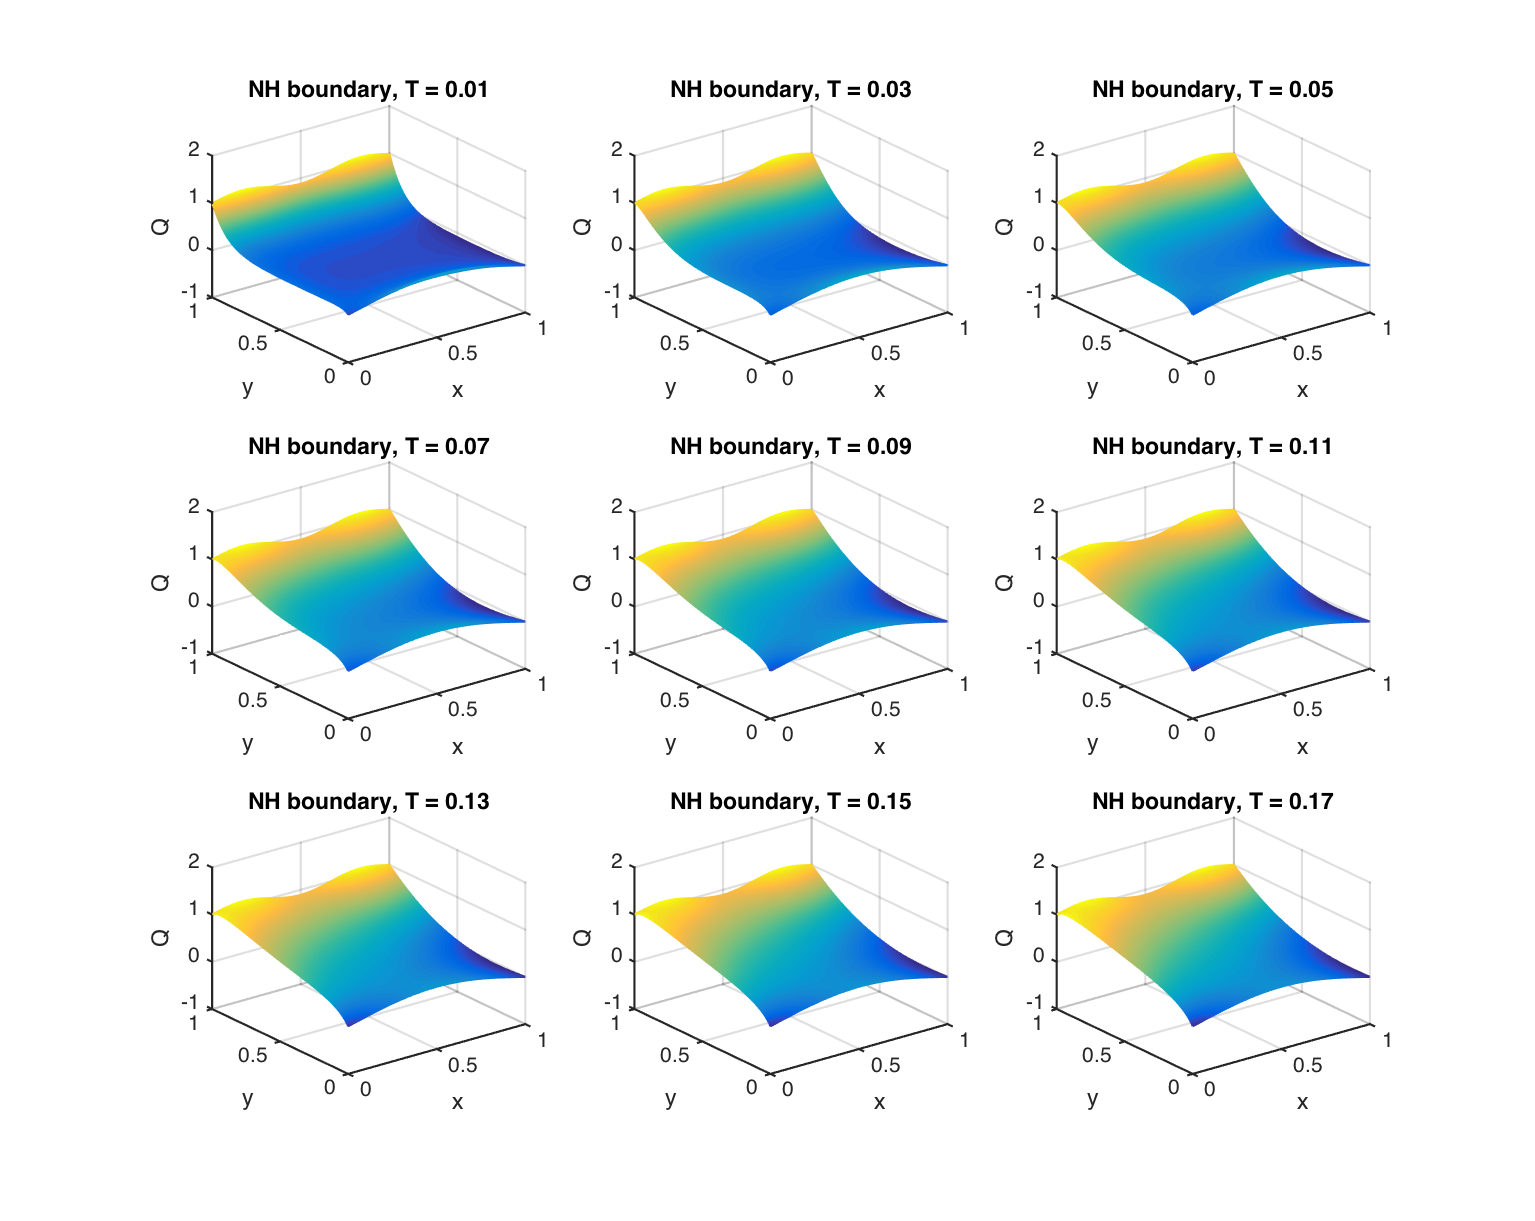
\includegraphics[scale=.6]{boundConv.eps}
\caption{Results with Non-homogeneous B.C.'s}
\label{fig:digraph}
\end{figure}

We used the given boundary conditions and the results are given in figure (6). We can see the boundary conditions given at $y=0$ and $y=1$. We can also see the evolution of the temperature. First, the gradients are really steep near the boundaries because the initial condition is zero. Then, the conduction acts and the gradients become less steep.

Let us now look at the convergence. Let us define : 
$$R = log_3(\frac{Q_h-Q_{h/3}}{Q_{h/3}-Q_{h/9}})$$

Where $Q_h$ is our solution evaluated at $(0.95,0.9)$ (it is no longer a good idea to use a boundary points because of the Dirichlet condition) at $t=0.2$ for a grid such that $h = \Delta x = \Delta y$. We get the following table : 
\begin{center}
\begin{tabular}{|c|c|c|c|}
\hline 
h & $\frac{1}{10}$ & $\frac{1}{30}$ & $\frac{1}{90}$ \\ 
\hline 
R & 2.1555 & 2.0284 & 2.0033 \\ 
\hline 
\end{tabular} 
\end{center}

Once again, we can conclude that we have an order 2 convergence in space.

Let us now look at the convergence. With the same definition for $H$ as in section 5.1, we get the following table :
\begin{center}
\begin{tabular}{|c|c|c|c|}
\hline 
$\Delta t$ & 0.08 & 0.04 & 0.02 \\ 
\hline 
H & 1.1255 & 1.0951 & 1.0587 \\ 
\hline 
\end{tabular} 
\end{center}

We find back the order 1 convergence for implicit Euler.\\

Finally, a word about conservation. Let us first look at the left and right boundaries. There,  $q_x=-1$ so the heat flux is the same at the left and right boundaries. However, at the upper and lower boundaries, we have Dirichlet conditions, meaning that there is also a heat flux at those boundaries but they are not equivalent. Thus, we no longer have conservation. It is easy to see on the plots. Even though the heat source is not zero, the temperature distribution looks like it is reaching a stationary state. The heat has thus to get out of the domain.